%%% Copyright (C) 2018 Vincent Goulet
%%%
%%% Ce fichier fait partie du projet
%%% «Rédaction avec LaTeX»
%%% http://github.com/vigou3/formation-latex-ul
%%%
%%% Cette création est mise à disposition selon le contrat
%%% Attribution-Partage dans les mêmes conditions 4.0
%%% International de Creative Commons.
%%% http://creativecommons.org/licenses/by-sa/4.0/

\section{Principes de base}

\subsection{Règles de saisie}

\begin{frame}[fragile=singleslide]
  \frametitle{Rédaction}

  L'apparence du document est prise en charge par {\LaTeX} et
  il est généralement préférable de ne pas la modifier.

  \begin{itemize}
  \item On se concentre sur le \alert{contenu} et la \alert{structure} du
    document
      \bigskip
      \begin{tabbing}
        titre de section \qquad\= \faArrowRight \qquad\= \verb|\section{titre}| \\[6pt]
        emphase \> \faArrowRight \> \verb|\emph{texte}|
      \end{tabbing}
      \bigskip
  \item Mots séparés par une ou plusieurs \alert{espaces}
  \item Paragraphes séparés par une ou plusieurs \alert{lignes blanches}
  \item Utilisation de \alert{commandes} pour indiquer la structure du texte
  \end{itemize}
\end{frame}

\subsection{Structure d'un fichier}

\begin{frame}[fragile]
  \frametitle{Structure d'un document {\LaTeX}}

  Un fichier source {\LaTeX} est toujours composé de deux parties.

  \hfill
  \begin{minipage}{0.75\linewidth}
\begin{lstlisting}[emph={documentclass,begin,end,document}]
\documentclass[11pt,french]{article}
  \usepackage{babel}
  \usepackage[autolanguage]{numprint}
  \usepackage[utf8]{inputenc}
  \usepackage[T1]{fontenc}

\begin{document}

Lorem ipsum dolor sit amet, consectetur
adipiscing elit. Donec quam nulla, bibendum
vitae ipsum vel, fermentum pellentesque orci.

\end{document}
\end{lstlisting}
  \end{minipage}

  \begin{textblock*}{\linewidth}(0mm,0mm)
    \begin{picture}(0,0)
      \thicklines\color{blue}
      \onslide<2>{\put(120,-138){\dashbox{2}(285,76){}}}
      \onslide<3>{\put(120,-248){\dashbox{2}(285,104){}}}
      \onslide<2>{\put(46,-103){préambule}}
      \onslide<3>{\put(46,-198){\parbox{25mm}{corps du\\ document}}}
    \end{picture}
  \end{textblock*}
\end{frame}

\subsection{Classes et paquetages}

\begin{frame}[fragile]
  \frametitle{Classe de document}

  La première commande du préambule est normalement la déclaration de
  la classe de la forme
\begin{lstlisting}
\documentclass`\oarg{options}\marg{classe}'
\end{lstlisting}

  \begin{itemize}
  \item Principales classes
    \begin{quote}
      \class{article, report, book, letter} \\
      {\color{alert} \class{memoir}} \\
      {\color{alert} \class{ulthese}}
    \end{quote}
  \item Principales options
    \begin{quote}
      \texttt{10pt, {\color{alert} 11pt}, 12pt} \\
      \texttt{oneside, twoside} \\
      \texttt{openright, openany} \\
      {\color{alert} \texttt{article}} (classe \class{memoir})
    \end{quote}
  \end{itemize}
\end{frame}

\begin{frame}[fragile=singleslide]
  \frametitle{Paquetages}
  \begin{itemize}
  \item Permettent de modifier des commandes ou d'ajouter des
    fonctionnalités au système
  \item Chargés dans le préambule avec
    \begin{lstlisting}
\usepackage`\marg{paquetage}'
\usepackage`\oarg{options}\marg{paquetage}'
\usepackage`\marg{paquetage1,paquetage2,...}'
    \end{lstlisting}
  \end{itemize}
\end{frame}

\subsection{[~Exercice~]}

\begin{exercice}
  Utiliser le fichier \fichier{exercice\_classe+paquetages.tex}.

  \begin{enumerate}
  \item Compiler le fichier tel que fourni.
  \item Changer la police du document pour 11~points, puis 12~points.
    Observer l'effet sur les marges et sur la coupure automatique des
    mots.
  \item Activer le paquetage \pkg{icomma} en supprimant le symbole \%
    au début de la ligne dans le préambule. Observer l'effet sur la
    formule mathématique.
  \item Charger le paquetage \pkg{numprint} avec l'option
    \verb=autolanguage= (\emph{après} le paquetage \pkg{babel}). Dans
    le code source de la formule mathématique, changer
\begin{lstlisting}
10 000
\end{lstlisting}
    pour
\begin{lstlisting}
\nombre{10000}
\end{lstlisting}
    et observer le résultat.
  \end{enumerate}
\end{exercice}

\subsection{Commandes et environnements}

\begin{frame}[fragile=singleslide]
  \frametitle{Commandes}
  \begin{itemize}
  \item Débutent toujours par \bs
  \item Formes générales:
\begin{lstlisting}
\`\meta{nomcommande}\oarg{arg\_optionnel}\marg{arg\_obligatoire}'
\`\meta{nomcommande}'*`\oarg{arg\_optionnel}\marg{arg\_obligatoire}'
\end{lstlisting}
   \item Commande sans argument: le nom se termine par tout
    caractère qui n'est pas une lettre (y compris l'espace!)
  \item Portée d'une commande limitée à la zone entre \verb={ }=
  \end{itemize}
\end{frame}

\begin{frame}[fragile=singleslide]
  \frametitle{Environnements}
  \begin{itemize}
  \item Délimités par
\begin{lstlisting}
\begin`\marg{environnement}'
   ...
\end`\marg{environnement}'
    \end{lstlisting}
  \item Contenu de l'environnement traité différemment du reste du texte
  \item Changements s'appliquent uniquement à l'intérieur de
    l'environnement
  \end{itemize}
\end{frame}

\subsection{Commentaires}

\begin{frame}[fragile=singleslide]
  \frametitle{Commentaires}
  \begin{itemize}
  \item Le symbole \verb=%= sert à identifier les commentaires dans
    le code source
  \item Tout ce qui suit \verb=%= sur la ligne est ignoré
    \begin{demo}
      \begin{texample}
\begin{lstlisting}
texte % ignoré par LaTeX
\end{lstlisting}
        \producing
        texte % ignoré par LaTeX
      \end{texample}
    \end{demo}
  \end{itemize}
\end{frame}

\subsection{[~Exercice~]}

\begin{exercice}
  Modifier le fichier \fichier{exercice\_commandes.tex} afin de
  produire le texte ci-dessous.

  \bigskip
  \centering
  \fbox{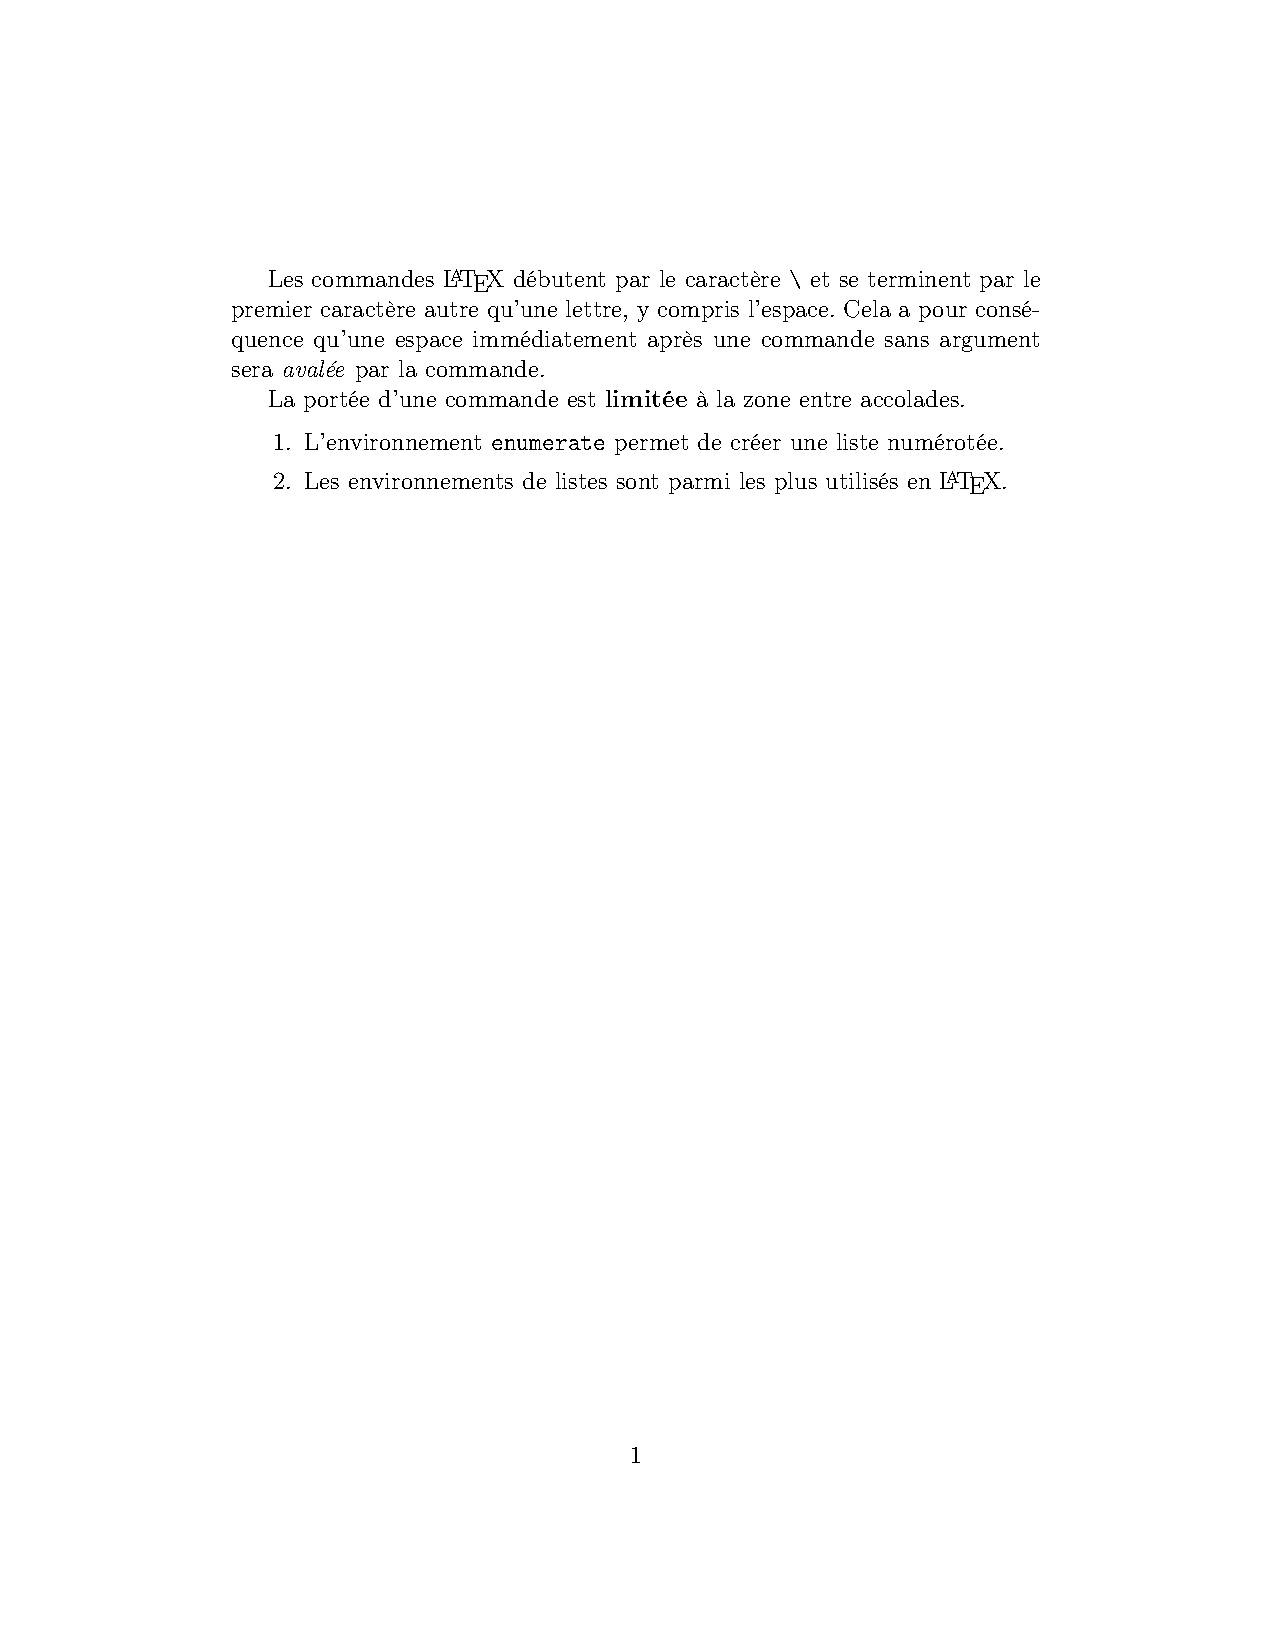
\includegraphics[viewport=108 551 502 665,%
    clip=true,width=0.9\linewidth]{exercice_commandes-solution}}
\end{exercice}

\subsection{Caractères spéciaux}

\begin{frame}[fragile=singleslide]
  \frametitle{Caractères réservés}

  \begin{itemize}
  \item Caractères réservés par {\TeX}:
    \begin{quote}
      \verb=# $ & ~ _ ^ % { }=
    \end{quote}
  \item Pour les utiliser, précéder par \bs
  \item On écrira donc
    \begin{demo}
      \begin{texample}
\begin{lstlisting}
L'augmentation de 2~\$
représente une hausse
de 5~\%.
\end{lstlisting}
        \producing
        L'augmentation de 2~\$ représente une
        hausse de 5~\%.
      \end{texample}
    \end{demo}
  \end{itemize}
\end{frame}

\begin{frame}[fragile=singleslide]
  \frametitle{Espaces, guillemets et tirets}
  \begin{itemize}
  \item Espace insécable
\begin{lstlisting}
M.~Tremblay me doit 200~\$.
\end{lstlisting}
  \item Guillemets
    \begin{demo}
      \begin{texample}
\begin{lstlisting}[escapeinside={}]
``guillemets anglais''
\end{lstlisting}
        \producing
        ``guillemets anglais''
      \end{texample}
      \begin{texample}
\begin{lstlisting}
«guillemets français»
\end{lstlisting}
        \producing
        «guillemets français»
      \end{texample}
   \end{demo}
  \item Tiret, tiret demi-cadratin, tiret cadratin
    \begin{demo}
      \begin{minipage}{0.15\linewidth}
        \begin{texample}
\begin{lstlisting}
-
\end{lstlisting}
          \producing
          -
        \end{texample}
      \end{minipage}
      \hfill
      \begin{minipage}{0.15\linewidth}
        \begin{texample}
\begin{lstlisting}
--
\end{lstlisting}
          \producing
          --
        \end{texample}
      \end{minipage}
      \hfill
      \begin{minipage}{0.15\linewidth}
        \begin{texample}
\begin{lstlisting}
---
\end{lstlisting}
          \producing
          ---
        \end{texample}
      \end{minipage}
      \hfill
    \end{demo}
  \item Détails additionnels à la section~2.9 du document de référence
  \end{itemize}
\end{frame}

\begin{frame}[fragile]
  \frametitle{{\LaTeX} en français}

  Il faut charger un certain nombre de paquetages pour franciser \LaTeX.

  \begin{itemize}
  \item \pkg{babel}: traduction des mots-clés prédéfinis,
    typographie française, coupure de mots, document multilingue
  \item \pkg{inputenc} et \pkg{fontenc}: lettres accentuées dans le
    code source (pdf{\LaTeX} seulement)
  \item \pkg{icomma}: virgule comme séparateur décimal
  \item \pkg{numprint}: espace comme séparateur des milliers
  \end{itemize}
\end{frame}

%%% Local Variables:
%%% TeX-master: "formation-latex-ul-diapos"
%%% TeX-engine: xetex
%%% coding: utf-8
%%% End:
